\subsection{Khả năng phân loại của ánh xạ đặc trưng tuyến tính từng phần}
SVM với ánh xạ đặc trưng tuyến tính từng phần (PWL) tạo ra một ranh giới tuyến tính từng phần và thừa hưởng các đặc tính tốt của SVM. Khả năng phân loại của PWL-SVM liên quan đến công thức cụ thể của \( \phi_m(x) \).

\noindent Công thức đơn giản nhất là
\begin{align}
    \phi_m(x) = \max\{0, x(i_m) - q_m\},
    \label{eq:phi_m}
\end{align}
trong đó \( q_m \in \mathbb{R} \) và \( i_m \in \{1, \ldots, n\} \) biểu thị thành phần được sử dụng trong \( \phi_m(x) \). Sử dụng \eqref{eq:phi_m} làm ánh xạ đặc trưng, một bộ phân loại tuyến tính từng phần cộng có thể được xây dựng. Các điểm thay đổi của ranh giới phân loại tuyến tính từng phần nên được đặt tại các ranh giới của các vùng con và các ranh giới được cung cấp bởi \eqref{eq:phi_m} bị giới hạn là các đường song song với một trong các trục.

Vì các ranh giới của các vùng con được định nghĩa bởi \eqref{eq:phi_m} không đủ linh hoạt, một số bộ phân loại mong muốn không thể đạt được. Để mở rộng khả năng phân loại, ta nên mở rộng \eqref{eq:phi_m} thành
\begin{align}
    \phi_m(x) = \max\{0, p_m^T x - q_m\},
    \label{eq:phi_m_extend}
\end{align}
trong đó \( p_m \in \mathbb{R}^n, q_m \in \mathbb{R} \). Công thức này được gọi là một siêu phẳng bản lề - Hinging Hyper Plane(HH [16]) và các ranh giới của các vùng con được cung cấp bởi siêu phẳng là các đường xuyên suốt miền, linh hoạt hơn so với \eqref{eq:phi_m}. Để có được một bộ phân loại tuyến tính từng phần với khả năng phân loại mạnh mẽ hơn, ta có thể thêm nhiều hàm tuyến tính theo cách sau
\[
\phi_m(x) = \max\{0, p_{m1}^T x - q_{m1}, p_{m2}^T x - q_{m2}, \ldots\}.
\]
Khả năng phân loại được mở rộng cùng với sự gia tăng của các hàm tuyến tính được sử dụng trong \(\max\{\}\). Như đã chứng minh trong Định lý \ref{thm:pwl_funtion}, một ranh giới tuyến tính từng phần bất kỳ trong không gian n-chiều có thể được thực hiện bằng cách sử dụng \(n\) hàm tuyến tính, tức là
\begin{align}
    \phi_m(x) = \max\{0, p_{m1}^T x - q_{m1}, p_{m2}^T x - q_{m2}, \ldots, p_{mn}^T x - q_{mn}\},
    \label{eq:use_n_linear}
\end{align}
Theo ký hiệu trong [18], chúng ta gọi \eqref{eq:use_n_linear} là ánh xạ đặc trưng siêu phẳng bản lề tổng quát - Generalized Hinging HyperPlane (GHH).

\subsection{Tham số trong ánh xạ đặc trưng tuyến tính từng phần}
Giống như các ánh xạ đặc trưng phi tuyến hoặc các hạt nhân khác, ánh xạ đặc trưng tuyến tính từng phần có một số tham số phi tuyến, có ảnh hưởng lớn đến hiệu suất phân loại nhưng khó điều chỉnh tối ưu. Để có được các tham số hợp lý cho ánh xạ đặc trưng tuyến tính từng phần, ta nghiên cứu ý nghĩa hình học của các tham số. Từ định nghĩa của một tập tuyến tính từng phần, miền được chia thành các vùng con \(\om_k\), trong mỗi vùng con đó tập tuyến tính từng phần bằng một siêu phẳng. Nói chung, các tham số trong ánh xạ đặc trưng tuyến tính từng phần xác định cấu trúc vùng con và siêu phẳng trong mỗi vùng con được thu được bằng kỹ thuật SVM.

\begin{figure}
    \centering
    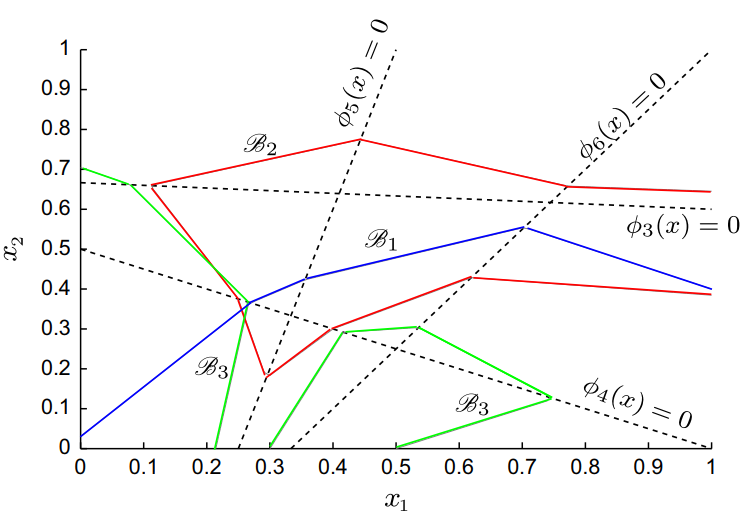
\includegraphics[width=0.9\textwidth]{images/bound_of_subregions.png}
    \caption[Ranh giới của các vùng con]{\textbf{Các ranh giới của các vùng con} cho \eqref{eq:phi_m} và các ranh giới phân loại liên quan.}
    \label{fig:bound_of_subregions}
\end{figure}

Xét lại tập dữ liệu hai mặt trăng được hiển thị trong Hình \ref{fig:moon_data}. Ranh giới bao gồm ba đoạn nằm trong vùng con \(\om_k\) như minh họa trong Hình \ref{fig:pwl_boundary}. Để xây dựng bộ phân loại mong muốn, ta đặt
\[
\phi_1(x) = x(1), \quad \phi_2(x) = x(2),
\]
\[
    \phi_3(x) = \max\{0, x(2) - \frac{1}{3}\}, \quad \phi_4(x) = \max\{0, x(2) - \frac{2}{3}\},
\]
tức là, ta sử dụng ánh xạ đặc trưng \eqref{eq:phi_m} với \(i_1 = 1, q_1 = 0, i_2 = 2, q_2 = 0, i_3 = 2, q_3 = \frac{1}{3},\) và \(i_4 = 2, q_4 = \frac{2}{3}\). Tiếp theo giải PWL-C-SVM hoặc PWL-LS-SVM dẫn đến \(\text{w}_0, \ldots, \text{w}_4\), xác định một ranh giới tuyến tính từng phần
\(
\text{w}_0 + \sum_{m=1}^{4} \text{w}_m f_m(x) = 0.
\)
Trong ví dụ này, dựa vào một số kiến thức trước đó đã được biết, các tham số hợp lý cho một ánh xạ đặc trưng tuyến tính từng phần có thể được tìm thấy một cách hiệu quả. Trong các vấn đề hộp đen, chúng ta đặt các tham số của \eqref{eq:phi_m} bằng cách chia đều miền trên mỗi trục thành nhiều đoạn.

Đối với các ánh xạ đặc trưng tuyến tính từng phần khác, chúng ta sử dụng các tham số ngẫu nhiên. Các ranh giới của các đoạn được cung cấp bởi \eqref{eq:phi_m_extend} là các siêu phẳng \(p_m^T x + q_m = 0\). Để có được \(p_m \in \mathbb{R}^n\) và \(q_m \in \mathbb{R}\), trước tiên chúng ta tạo ra \(n\) điểm trong miền với phân phối đều, sau đó chúng ta chọn \(p_m(1)\) từ \(\{1, -1\}\) với xác suất bằng nhau, và tính \(q_m\) và các thành phần khác của \(p_m\) sao cho các điểm được tạo ra nằm trong \(p_m^T x + q_m = 0\). Các tham số thu được theo cách này có thể cung cấp các ranh giới phân loại linh hoạt.  

Hình \ref{fig:bound_of_subregions} cho thấy các ranh giới của các vùng con cho liên quan đến ánh xạ đặc trưng tuyến tính tưng phần được tạo ngẫu nhiên. Bốn đường nét đứt tương ứng với \(f_3(x) = 0\), \(f_4(x) = 0\), \(f_5(x) = 0\), và \(f_6(x) = 0\), tương ứng. Ranh giới phân loại là \(\mathcal{B} = \{x : w_0 + \sum_{m=1}^{6} w_m f_m(x) = 0\}\). \(\mathcal{B}_1\) với \(w_0 = -1.5, w_1 = 0.5, w_2 = 0.9, w_3 = 0.7, w_4 = 0.8, w_5 = 0.1, w_6 = 0.33\), \(\mathcal{B}_2\) với \(w_0 = -0.5, w_1 = -0.5, w_2 = 1, w_3 = -1, w_4 = 0.8, w_5 = -0.25, w_6 = 0.33\), và \(\mathcal{B}_3\) với \(w_0 = -0.5, w_1 = 1, w_2 = -2, w_3 = 1, w_4 = 4, w_5 = -0.75, w_6 = 0.67\) được minh họa bằng các đường màu đỏ, xanh dương, và xanh lá cây, cho thấy sự linh hoạt của ranh giới phân loại, có thể là lồi (\(\mathcal{B}_1\)), không lồi (\(\mathcal{B}_2\)), và không kết nối (\(\mathcal{B}_3\)).
\begin{align}
    f_1(x) &= x(1), \quad f_2(x) = x(2), \notag \\
    f_3(x) &= \max\{0, x(1) + 1.5 x(2) - 1.0\}, \notag \\
    f_4(x) &= \max\{0, x(1) + 2 x(2) - 1.0\}, \notag \\
    f_5(x) &= \max\{0, -x(1) + 0.25 x(2) + 0.25\}, \notag \\
    f_6(x) &= \max\{0, -x(1) + 0.67 x(2) + 0.33\}.
    \label{eq:random_subregions}
\end{align}
Ba ranh giới phân loại có thể tương ứng với các nhóm \(\text{w}_m\) khác nhau được hiển thị. Có thể thấy sự linh hoạt của các bộ phân loại tiềm năng, từ đó bộ phân loại tối ưu có thể được chọn ra bằng SVM. Trong hầu hết các trường hợp, hiệu suất phân loại là thỏa đáng, nếu không, chúng ta có thể tạo ra một nhóm tham số khác. Tương tự, các tham số của \eqref{eq:use_n_linear} có thể được tạo ra và các vùng con kết quả cung cấp các ranh giới phân loại linh hoạt.